\noindent\fcolorbox{boxrule}{boxbg}{\begin{minipage}{\dimexpr\textwidth-2\fboxsep-2\fboxrule\relax}
\small
\textbf{What I ran.} CertLI end to end on two ColBERT models (ColBERTv2, AnswerAI-ColBERT-small) and two BEIR corpora (SciFact, NFCorpus): corpus-mean shift (Lemma 1), low-rank-plus-sparse token codes, interval MaxSim bounds (Lemma 2), bound-ordered exact refinement, and a risk-controlled variant calibrated with Learn-then-Test \cite{3}. Ground truth is exact MaxSim against every document, so no number below depends on a candidate generator.

\vspace{3pt}
\textbf{Findings.}
\begin{enumerate}[leftmargin=1.4em,itemsep=3pt]
\item \textbf{The math holds on real models.} The mean shift left every ranking unchanged (max score deviation $4.4\times10^{-6}$, identical top-100 for all queries), and the interval bounds were never violated in 50.3M (query, document) checks.
\item \textbf{Deterministic certificates do not pay off at useful compression.} With codes at about one third of the fp16 index, proving the exact top-10 still requires scoring 79\% to 95\% of the corpus at full precision for ColBERTv2 and 100\% for AnswerAI-small (Fig.~\ref{fig:reads}, grey).
\item \textbf{The reason is measurable.} The coding error points in a near-random direction relative to the query, so the realised error is a median 5\% of its worst-case bound. Meanwhile the median gap between the 10th and 11th exact scores is 0.08 (ColBERTv2) and below 0.01 (AnswerAI), against a mean interval slack of 5 to 11. No worst-case bound separates scores that close.
\item \textbf{Calibrated certificates work.} Shrinking the same intervals by a factor chosen with Learn-then-Test (wrong top-10 on at most 5\% of queries, with 90\% confidence) scores 1.4\% of the corpus on ColBERTv2/SciFact, with 0.7\% of held-out queries wrong. Caveat: a fixed rerank depth calibrated the same way is equally cheap, so the gain comes from calibration, not yet from per-query adaptivity. A perfect stopping rule would read 3 to 7 times less: that is the headroom.
\item \textbf{A geometric finding relevant to EigenLI \cite{2}.} AnswerAI-small tokens share one dominant direction (random tokens from different documents have cosine 0.82 to 0.84). Removing it is exactly rank-safe for MaxSim, but not for spectral scores: removing it from documents only collapses an EigenLI-style score from 68.0 to 1.6 nDCG@10; removing it from both sides is neutral to helpful (+2.2 at $k=32$).
\end{enumerate}
\end{minipage}}

\vspace{6pt}
\begin{figure}[H]
\centering
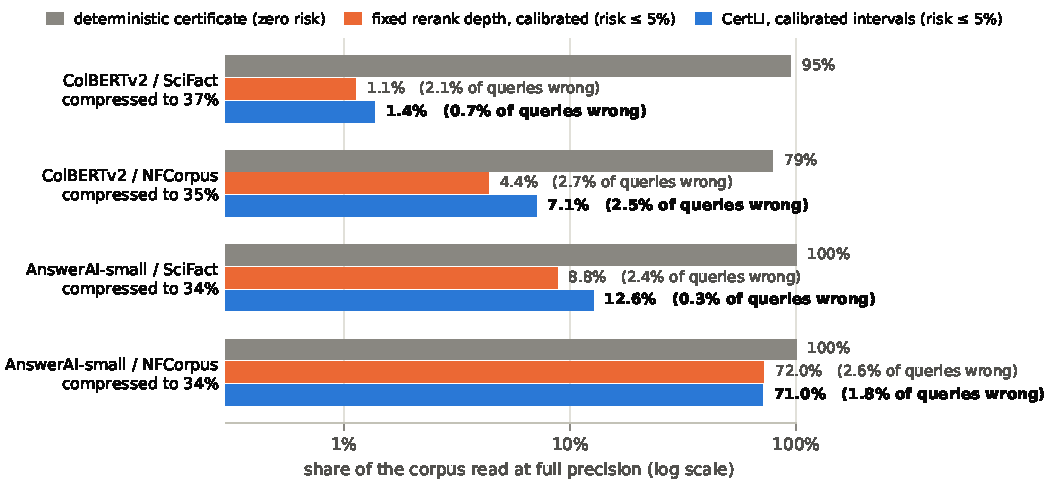
\includegraphics[width=\textwidth]{../figs/f1_reads.pdf}
\caption{Share of the corpus that must be scored at full precision to return the top-10, with codes at about one third of the fp16 index size. Grey: deterministic certificate (exact top-10 guaranteed). Blue: the same intervals shrunk by a factor chosen with Learn-then-Test so that $\Pr[\text{top-10}\ne\text{exact}]\le5\%$ with confidence 90\%. Orange: a fixed rerank depth calibrated the same way. In brackets: realised share of held-out queries whose top-10 differs from exact MaxSim (mean over 200 random calibration/test splits).}
\label{fig:reads}
\end{figure}

%=====================================================================
\section{Setup}
\textbf{Models.} ColBERTv2 \cite{6} (128-d tokens) and AnswerAI-ColBERT-small-v1 (96-d), encoded with PyLate using each model's prefixes, \texttt{[MASK]} query expansion to 32 tokens and the punctuation skiplist; documents cut at 300 tokens. \textbf{Data.} BEIR SciFact (5,183 documents, 300 test queries) and NFCorpus (3,633 documents, 323 test queries). \textbf{Scoring.} Exact MaxSim $C(Q,D)=\sum_i\max_j\langle q_i,d_j\rangle$ over the whole corpus; nDCG@10 as in BEIR. \textbf{Codes.} Each document is shifted by the corpus mean $\mu$ and coded in its own eigenbasis ($k\le32$, chosen per document to minimise bytes); tokens with residual above $\tau$ are kept verbatim and the rest are pooled into clusters of radius $\le\varepsilon$, each with its own radii. $\tau,\varepsilon$ are in units of the RMS shifted-token norm. With the same bounds I also certify POOL (clusters in the full space, no subspace) and PLAID-style residual codes \cite{8} (centroid plus $b$-bit residual per dimension, with a 1-byte error radius per token). \textbf{Cost.} Given bounds $[L_D,U_D]$ and the exact 10th score $s_{(10)}$, any correct method must score every $D$ with $U_D\ge s_{(10)}$, and bound-ordered refinement scores exactly those \cite{4}. I report that count as a share of the corpus. \textbf{Hardware.} 2 CPU cores, 7\,GB RAM, no GPU.

%=====================================================================
\section{Sanity checks}
\begin{table}[H]
\centering\small
\caption{Exact MaxSim reproduces published nDCG@10 (in brackets). IDF: token-importance weights as in \cite{1}, change in brackets. Lemma 1: shifting all document tokens by the corpus mean moves every score of a query by the same constant. Per-document centring, the obvious alternative, is not rank-safe.}
\label{tab:sanity}
\begin{tabular}{llccccc}
\toprule
Model & Data & \hd{nDCG@10\\(published)} & \hd{IDF-weighted\\nDCG@10} & \hd{Lemma 1: max\\score deviation} & \hd{Same\\top-100} & \hd{Per-doc centring\\nDCG@10} \\
\midrule
\tabin{../tables/k1.tex}
\bottomrule
\end{tabular}
\end{table}
Exact MaxSim matches the published numbers within 0.6 points, so encoders and evaluation are right. IDF weights help ColBERTv2 on SciFact ($+1.7$) and hurt AnswerAI-small ($-1.6$): useful token importance is model specific. Lemma 1 holds to float32 rounding. Centring each document by its own mean collapses AnswerAI-small (74.5 to 37.7), a first sign of its anisotropy.

%=====================================================================
\section{Results}
\subsection{The low-rank-plus-sparse structure is real}
\begin{table}[H]
\centering\small
\caption{Geometry of document token sets. Mean cosine between random tokens from different documents. Energy held by the top-16 eigenvectors of each document, and effective rank, before / after the shift. $|\cos(v_1,\mu)|$: alignment of each document's leading eigenvector with the corpus mean. Last two columns: how the residual after a rank-16 projection depends on token IDF.}
\label{tab:geom}
\begin{tabular}{llccccccc}
\toprule
Model & Data & $\nrm{\mu}$ & \hd{Token\\cosine} & \hd{Top-16\\energy \%} & \hd{Effective\\rank} & $|\cos(v_1,\mu)|$ & \hd{Spearman\\(IDF, residual)} & \hd{Residual, top /\\bottom IDF decile} \\
\midrule
\tabin{../tables/k2.tex}
\bottomrule
\end{tabular}
\end{table}
After the shift, 16 directions hold 74\% to 76\% of each document's energy. What is left concentrates on rare tokens: the residual grows with IDF (Spearman 0.45 to 0.55) and is 2.0 to 2.5 times larger in the top IDF decile than in the bottom one. This is the structure CertLI assumes, and the reason rare tokens are kept verbatim. AnswerAI-small is strongly anisotropic: its corpus mean has norm 0.90 to 0.92 for unit-norm tokens, each document's leading eigenvector is that mean ($|\cos|=0.99$), and the effective rank of a document rises from about 2.5 to about 29 once it is removed.

\subsection{Deterministic certificates read almost everything}
\begin{table}[H]
\centering\small
\caption{Share of the corpus scored at full precision to certify the exact top-10, in \% (code size as \% of fp16 in brackets). Last column: bound violations over all configurations run.}
\label{tab:cert}
\begin{tabular}{llcccccc}
\toprule
& & \multicolumn{4}{c}{low-rank + sparse, $(\tau,\varepsilon)$} & & \\
\cmidrule(lr){3-6}
Model & Data & $(0.3,0.25)$ & $(0.5,0.25)$ & $(0.5,0.45)$ & \hd{$(0.5,0.45)$,\\global radii} & \hd{POOL\\$\varepsilon=0.45$} & \hd{Violations\\/ checks} \\
\midrule
\tabin{../tables/k3.tex}
\bottomrule
\end{tabular}
\end{table}
No bound was violated, so bound-ordered refinement returns the exact top-10 by construction. The cost is the problem: the largest code (72\% of fp16) still scores 39\% of SciFact for ColBERTv2; at about one third of fp16 it scores 79\% to 95\%; for AnswerAI-small, everything. Two design choices do matter: per-cluster radii (global radii push 95\% to 100\%), and the subspace, since POOL needs 59\% of fp16 for the same cost that the low-rank code reaches at 40\% to 42\%. A 1-bit PLAID-style code (8\% of fp16, AnswerAI/NFCorpus) also scores 100\%.

\subsection{Why: the bound pays for a worst case that almost never happens}
\begin{figure}[H]
\centering
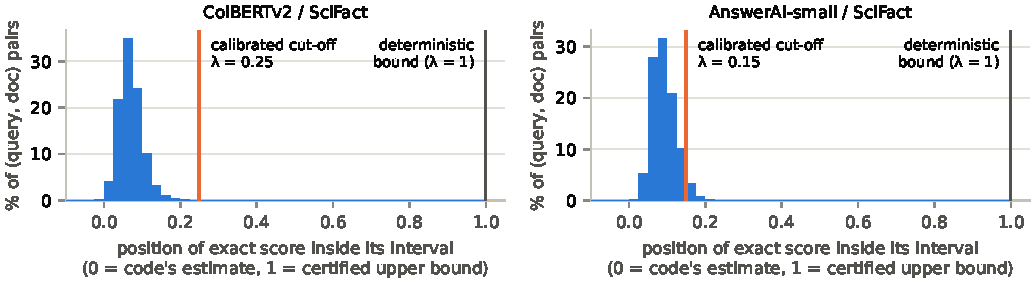
\includegraphics[width=\textwidth]{../figs/f2_position.pdf}
\caption{Where the exact score falls inside its certified interval, over all (query, document) pairs (codes at about one third of fp16 size). The deterministic certificate must cover position 1; the cut-off chosen by Learn-then-Test sits just past where the mass ends.}
\label{fig:pos}
\end{figure}
\begin{table}[H]
\centering\small
\caption{Token level: RMS cosine between a query token's off-subspace component and the coding residual (isotropic prediction $1/\sqrt{\dim-k}$ in brackets), and the realised deviation as a share of its bound (median / 99th percentile). Document level: median gap between the 10th and 11th exact scores, mean upper slack $U-S$, and 99th percentile / maximum position of the exact score inside its interval.}
\label{tab:why}
\begin{tabular}{llccccc}
\toprule
Model & Data & \hd{RMS cosine\\(isotropic)} & \hd{Deviation\\/ bound} & \hd{Top-10\\gap} & \hd{Mean\\slack} & \hd{Position\\p99 / max} \\
\midrule
\tabin{../tables/k4.tex}
\bottomrule
\end{tabular}
\end{table}
Two facts explain Table~\ref{tab:cert}. First, Lemma 2 charges each query token as if the coding error were aligned with it, but the error direction is close to random: its RMS cosine with the query is only 1.07 to 1.22 times the isotropic value. The realised deviation is therefore a median 5\% of its bound, and the exact score sits a median 5\% to 14\% of the way from the code's estimate to the upper bound, never beyond 62\% (Fig.~\ref{fig:pos}). Second, the top-10 is decided by tiny margins: the median gap between the 10th and 11th scores is 0.08 to 0.10 for ColBERTv2 and 0.003 to 0.009 for AnswerAI-small, against a mean slack of 5 to 11. To certify, the upper bounds of thousands of documents must fall below such a gap. Worst-case radii cannot do that; calibration exploits exactly the distance between worst and typical case.

\subsection{Calibrated certificates: same intervals, a statistical guarantee}
\begin{table}[H]
\centering\small
\caption{Learn-then-Test, $\alpha=0.05$, $\delta=0.1$, 200 random 50/50 calibration/test splits, loss $=\mathbf 1\{\text{top-10}\ne\text{exact}\}$. Share of the corpus scored, in \%; realised share of held-out queries with a wrong top-10 in brackets. Oracle: mean depth of a perfect per-query stopping rule.}
\label{tab:ltt}
\begin{tabular}{lllccccc}
\toprule
Model & Data & \hd{Code\\(size)} & Deterministic & \hd{Calibrated\\CertLI} & $\hat\lambda$ & \hd{Calibrated\\fixed depth} & Oracle \\
\midrule
\tabin{../tables/k5.tex}
\bottomrule
\end{tabular}
\end{table}
Calibration turns the slack into savings. The selected shrink factor $\hat\lambda$ is 0.15 to 0.40, consistent with Fig.~\ref{fig:pos}. On ColBERTv2/SciFact, CertLI scores 70 of 5,183 documents per query on average and returns a wrong top-10 on 0.7\% of held-out queries against the 5\% target (54 documents at $\alpha=0.10$). The realised error stays between 0.3\% and 2.5\% in all four settings. Two honest observations. (i) A fixed depth in the code's score order, calibrated the same way, is equally cheap or cheaper, at a higher realised error: today the gain comes from calibration, not from adaptivity. (ii) Adaptivity has real headroom: a perfect per-query rule scores 0.4\% to 14.4\%, 3 to 7 times less than the best fixed depth, and the oracle depth correlates with how crowded the scores near the 10th are (Spearman 0.36 to 0.69), which suggests a learnable stopping rule. AnswerAI/NFCorpus stays expensive (71\%) because its score gaps are the smallest (0.003).

\subsection{Side result: the shared direction and EigenLI}
\begin{table}[H]
\centering\small
\caption{SciFact, $k$ vectors per document (equal storage across columns): nDCG@10, with overlap with the exact top-10 in \% in brackets. Exact MaxSim next to the model name. EigenLI here is my re-implementation of the projection score $\sum_i\nrm{\Pi_D q_i}^2$, with $\Pi_D$ the top-$k$ eigenspace of the document's token second-moment matrix \cite{2}. Ward: hierarchical token pooling \cite{7}.}
\label{tab:eigen}
\begin{tabular}{lccccc}
\toprule
Model (exact) & $k$ & EigenLI & \hd{Mean removed,\\documents only} & \hd{Mean removed,\\documents and queries} & Ward pooling \\
\midrule
\tabin{../tables/k6.tex}
\bottomrule
\end{tabular}
\end{table}
Removing the corpus mean from documents only destroys AnswerAI-small (68.0 to 1.6 at $k=16$): queries keep their large shared component, which now falls outside every document's subspace and turns into noise. Removing it from both sides is neutral at $k=16$ and helps at $k=32$ (67.4 to 69.6), while for the less anisotropic ColBERTv2 it costs 1.1 to 3.3 points. So one-sided centring is free for MaxSim (Lemma 1) but not for quadratic scores, and the right treatment of the shared direction is model dependent. At equal storage EigenLI beats Ward pooling by 4.4 to 8.0 points in every cell.

%=====================================================================
\section{Takeaways and next steps}
\textbf{What worked.} Both lemmas are correct and cheap to apply; the low-rank-plus-sparse structure is real and saves about 30\% of bytes over plain clustering at equal certification cost; calibrated certificates give a statistical guarantee while scoring 1.4\% to 12.6\% of the corpus in three of four settings.

\textbf{What did not.} Deterministic certificates need most of the corpus at useful compression, because worst-case radii ignore that coding error is nearly isotropic and that top-10 margins are tiny. Per-query adaptive stopping does not yet beat a calibrated fixed depth.

\textbf{Next.} (1) \emph{Randomised radii}: apply a random rotation or subtractive dither \cite{5} before coding, so that the near-isotropy measured here becomes a property the index guarantees; the bound can then use concentration instead of Cauchy-Schwarz, giving a high-probability certificate without calibration data. (2) \emph{Learned stopping} from margin and density features, aimed at the 3 to 7 times headroom in Table~\ref{tab:ltt}. (3) \emph{Scale}: MS MARCO and LoTTE with PLAID candidate generation on GPU, certifying PLAID's own residual codes.

\textbf{Scope.} Small corpora (3.6k and 5.2k documents), CPU only, exhaustive exact scoring as ground truth, 150 to 162 calibration queries per split. EigenLI is my re-implementation, not the authors' code.

\section*{References}
{\small
[1] Archish S, A.\ Garg, K.\ Shiragur, N.\ Kayal. Incorporating token importance in multi-vector retrieval. AAAI 2026.\quad
[2] Archish S, S.\ Basu, A.\ Garg, R.\ Krishnaswamy, K.\ Shiragur. EigenLI: spectral approximations to late interaction. arXiv:2609.07561, 2026.\quad
[3] A.\ N.\ Angelopoulos, S.\ Bates, E.\ J.\ Cand\`es, M.\ I.\ Jordan, L.\ Lei. Learn then Test: calibrating predictive algorithms to achieve risk control. arXiv:2110.01052, 2021.\quad
[4] T.\ Seidl, H.-P.\ Kriegel. Optimal multi-step $k$-nearest neighbor search. SIGMOD 1998.\quad
[5] L.\ Schuchman. Dither signals and their effect on quantization noise. IEEE Trans.\ Communication Technology, 1964.\quad
[6] K.\ Santhanam, O.\ Khattab, J.\ Saad-Falcon, C.\ Potts, M.\ Zaharia. ColBERTv2: effective and efficient retrieval via lightweight late interaction. NAACL 2022.\quad
[7] B.\ Clavi\'e, A.\ Chaffin, G.\ Adams. Reducing the footprint of multi-vector retrieval with minimal performance impact via token pooling. arXiv:2409.14683, 2024.\quad
[8] K.\ Santhanam, O.\ Khattab, C.\ Potts, M.\ Zaharia. PLAID: an efficient engine for late interaction retrieval. CIKM 2022.}
